\documentclass[../../../../main.tex]{subfiles}

\begin{document}

\section*{東大理科 数学 1965 表紙・配点・概略}

\begin{itemize}
    \item 得点: 120 / 120 点
    \item 所要時間: 100 分 / 150 分
\end{itemize}

\subsection*{難易度・分野一覧}
\begin{enumerate}
    \item ベン図 (難易度: A)
    \item 計算 (難易度: B)
    \item 座標 (難易度: A)
    \item 座標 (難易度: B)
    \item 三角 (難易度: B)
    \item 立体 (難易度: A)
\end{enumerate}

\subsection*{各問のメモ・解答概要}
\begin{enumerate}
    \item ベン図: (1) 48 (2) 10 (3) 5 (4) 2
    \item (手書き解答詳細参照)
    \item 座標でおく: $\frac{2}{3}$
    \item 座標でおく: $k \le \sqrt{2}-1$ の時、$P$は$O$から $\frac{k+1}{12}$； $k \ge \sqrt{2}-1$ の時、$P$は$C$にすれば良い
    \item $\sin$に直して計算: $y = -3x - 1 + \frac{3}{2}\sqrt{3}\pi$, $y = -3x + \frac{3}{2}\pi$, $y = -3x + 1 - \frac{3}{2}\sqrt{3} + 2\pi$
    \item 分割して計算: $\frac{2}{3}\pi$
\end{enumerate}

\newpage

\section*{第2問}

\noindent
[\textbf{解}] $C$の高さを $h = 1600 + x\ \text{[m]}$ とおくと、題意より、下図で
\[
\text{BC}' = \sqrt{3}(x+A), \quad \text{BA}' = \sqrt{3}A, \quad \text{AC}' = \frac{x}{2-\sqrt{3}}
\]
$(A = 390, \tan 15^\circ = 2-\sqrt{3})$

\begin{center}
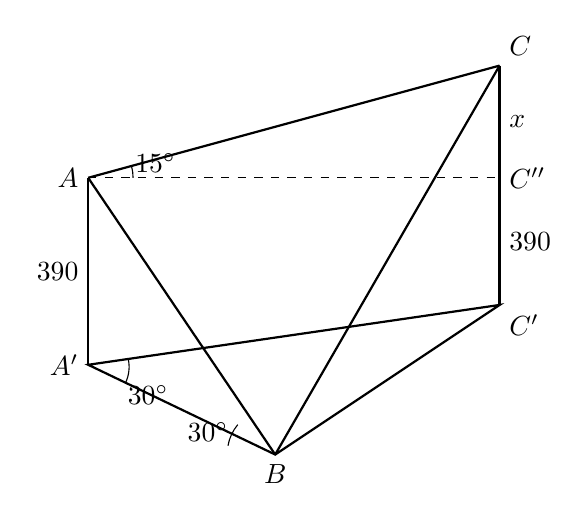
\begin{tikzpicture}[scale=0.95, >=stealth]
  % Coordinates
  \coordinate (Ap) at (0,0);
  \coordinate (A) at (0,2.5);
  \coordinate (B) at (2.5,-1.2);
  \coordinate (Cp) at (5.5,0.8);
  \coordinate (Cm) at (5.5,2.5);
  \coordinate (C) at (5.5,4.0);

  % Base triangle and vertical lines
  \draw[thick] (Ap) -- (B) -- (Cp) -- cycle;
  \draw[thick] (Ap) -- (A);
  \draw[thick] (Cp) -- (C);
  \draw[dashed] (A) -- (Cm);
  \draw[thick] (A) -- (C);
  \draw[thick] (A) -- (B);
  \draw[thick] (B) -- (C);

  % Labels for points
  \node[left] at (A) {$A$};
  \node[left] at (Ap) {$A'$};
  \node[below] at (B) {$B$};
  \node[below right] at (Cp) {$C'$};
  \node[right] at (Cm) {$C''$};
  \node[above right] at (C) {$C$};

  % Height labels
  \node[left] at (0, 1.25) {$390$};
  \node[right] at (5.5, 1.65) {$390$};
  \node[right] at (5.5, 3.25) {$x$};

  % Angle arcs and labels
  \draw (0.5,-0.24) arc (-25:12:0.5);
  \node at (0.8,-0.4) {$30^\circ$};

  \draw (2.0,-0.8) arc (140:170:0.6);
  \node at (1.6,-0.9) {$30^\circ$};

  \draw (0.6,2.5) arc (0:15:0.6);
  \node at (0.9,2.7) {$15^\circ$};
\end{tikzpicture}
\end{center}

\noindent
だから $\triangle A'BC'$ に余弦定理を用いて

\begin{center}
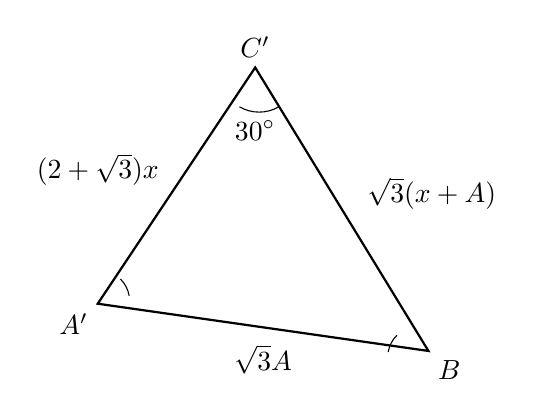
\begin{tikzpicture}[scale=1.0, >=stealth]
  \coordinate (Cp) at (2, 3);
  \coordinate (Ap) at (0, 0);
  \coordinate (B) at (4.2, -0.6);

  \draw[thick] (Ap) -- (B) -- (Cp) -- cycle;

  \node[above] at (Cp) {$C'$};
  \node[below left] at (Ap) {$A'$};
  \node[below right] at (B) {$B$};

  \node[left] at (0.9, 1.7) {$(2+\sqrt{3})x$};
  \node[right] at (3.3, 1.4) {$\sqrt{3}(x+A)$};
  \node[below] at (2.1, -0.4) {$\sqrt{3}A$};

  \draw (1.8, 2.5) arc (-120:-60:0.5);
  \node at (2.0, 2.2) {$30^\circ$};

  \draw (0.4, 0.1) arc (10:45:0.4);
  \draw (3.8, -0.4) arc (135:170:0.4);
\end{tikzpicture}
\end{center}

\noindent
セイリして
\begin{align*}
(\sqrt{3}A)^2 &= \left((2+\sqrt{3})x\right)^2 + 3(x+A)^2 - 2\sqrt{3}(2+\sqrt{3})x(x+A)\frac{\sqrt{3}}{2} \\
3A^2 &= (7+4\sqrt{3})x^2 + 3(x^2 + 2Ax + A^2) - (6+3\sqrt{3})(x^2 + Ax) \\
0 &= \left\{(7+4\sqrt{3}) + 3 - (6+3\sqrt{3})\right\}x^2 + (6A - 6A - 3\sqrt{3}A)x \\
0 &= (4+\sqrt{3})x^2 - 3\sqrt{3}Ax
\end{align*}
$x \neq 0$ より
\begin{align*}
(4+\sqrt{3})x &= 3\sqrt{3}A \\
x &= \frac{3\sqrt{3}}{4+\sqrt{3}}A \\
&= \frac{-9+12\sqrt{3}}{13}A \\
&= \frac{-9+12\cdot 1.732}{13} \cdot 390 \\
&= (-9+20.784) \cdot 30 \\
&= 353.52
\end{align*}
だから、$h = 1600 + 353.52 = 1953.52 \fallingdotseq 1954\text{ [m]}$

\end{document}
